\thispagestyle{plain}
	\section{Tecnología Existente}
		\subsection{Smartphone}
			\par 
				El teléfono inteligente (smartphone en inglés) es un tipo de ordenador de bolsillo que combina los elementos de una tablet con los de un teléfono celular. Sobre una plataforma informática móvil, con mayor capacidad de almacenar datos y realizar actividades, semejante a la de una minicomputadora, y con una mayor conectividad que un teléfono móvil convencional. El término inteligente, que se utiliza con fines comerciales, hace referencia a la capacidad de usarse como un computador de bolsillo, y llega incluso a reemplazar a una computadora personal en algunos casos.		
			\par \noindent
				Generalmente, los teléfonos con pantallas táctiles son los llamados teléfonos inteligentes, pero el soporte completo al correo electrónico parece ser una característica indispensable encontrada en todos los modelos existentes y anunciados desde 2007. Casi todos los teléfonos inteligentes también permiten al usuario instalar programas adicionales, habitualmente incluso desde terceros, hecho que dota a estos teléfonos de muchísimas aplicaciones en diferentes terrenos; sin embargo, algunos teléfonos son calificados como inteligentes aun cuando no tienen esa característica.			
			\par \noindent
				Entre otros rasgos comunes está la función multitarea, el acceso a Internet vía Wifi o redes 2G, 3G o 4G, función multimedia (cámara y reproductor de videos/mp3), a los programas de agenda, administración de contactos, acelerómetros, GPS y algunos programas de navegación, así como ocasionalmente la habilidad de y leer documentos de negocios en variedad de formatos como PDF y Microsoft Office.
			\par \noindent
				En la actualidad, el diseño de los smartphones es muy similar entre ellos: rectángular, con una o dos cámaras (tanto frontal como posterior) y algunos botones (generalmente 3, +volumen, -volumen y un botón para el bloqueo/encendido/apagado del dispositivo) ya que es totalmente táctil.
			\par \noindent
				Los sistemas operativos móviles más frecuentes utilizados por los teléfonos inteligentes son Android (de Google), iOS (de Apple) y Windows 10 (de Microsoft).
				
		\newpage
		\thispagestyle{plain}
		
		\subsection{Android}
			\par
				Android es un sistema operativo basado en el núcleo Linux. Fue diseñado principalmente para dispositivos móviles con pantalla táctil, como teléfonos inteligentes, tablets o tabléfonos; y también para relojes inteligentes, televisores y automóviles. Inicialmente fue desarrollado por Android Inc la cual fue fundado en 2003 por Andy Rubin, Rich Miner, Nick Sears y Chris White con el objetivo de desarrollar "dispositivos móviles que están al corriente de la ubicación y preferencias del usuario". En un principio la intención era desarrollar un sistema operativo avanzado para cámaras digitales, pero más tarde se cambió el foco al determinar que el mercado de las cámaras digitales no era lo suficientemente grande. Se redirigirían los esfuerzos a crear un sistema que pudiera competir con Symbian y Windows Mobile.
				
				\begin{figure}[h]
					\centering
					
\includegraphics[width=0.65\textwidth]{figure3_androidlogo.jpg}
					\caption{Un diseño preliminar para el logo de Android (izquierda) y el logo final (derecha)}
				\end{figure}
			
			\par \noindent
				 Posteriormente Google respaldó económicamente a Androind Inc. y más tarde, en 2005, la compró. Android fue presentado en 2007 junto la fundación del Open Handset Alliance (un consorcio de compañías de hardware, software y telecomunicaciones entre las que están Texas Instruments, Broadcom Corporation, Nvidia, Qualcomm, Samsung Electronics, Sprint Nextel, Intel, LG, Marvell Technology Group, Motorola, T-Mobile, etc) para avanzar en los estándares abiertos de los dispositivos móviles. El primer móvil con el sistema operativo Android fue el HTC Dream y se vendió en octubre de 2008. Los dispositivos de Android, hoy en día, venden más que las ventas combinadas de Windows Phone e iOS.
			
			\par \noindent
				La versión básica de Android es conocida como Android Open Source Project (AOSP).
			
			\begin{figure}[h]
				\centering
				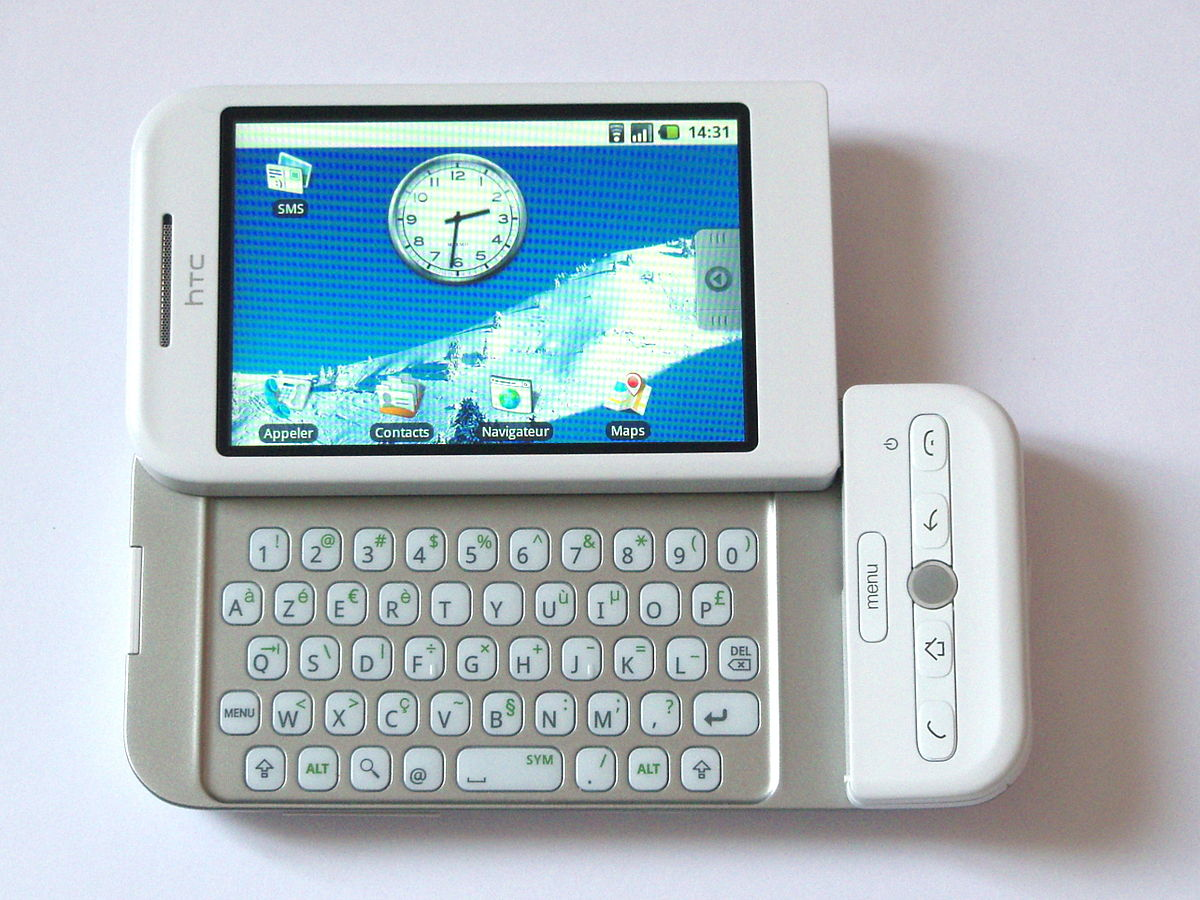
\includegraphics[width=8cm, height=6cm]{figura2_htcdream.jpeg}
				\caption{HTC Dream el primer teléfono con Android}
			\end{figure}
		
		\newpage
		\thispagestyle{plain}
		
		\subsubsection{Android 5.0 Lollipop}
			\par 
				Android Lollipop es una versión del sistema operativo para dispositivos móviles Android. Fue dada a conocer el 25 de junio de 2014 durante el Google I/O 2014 como Android L, Google I/O es una conferencia anual presentada por Google en sus oficinas en Mountain View, California.
				Los cambios más prominentes en Lollipop incluyen una interfaz de usuario rediseñada construida sobre un diseño de lenguaje responsivo denominado como "Material design", así como mejoras en el sistema de notificaciones que permiten que este sea accedido desde la pantalla de bloqueo, y mostrado junto con otras aplicaciones como banners en la parte superior de la pantalla. También se realizaron cambios internos para mejorar y optimizar el rendimiento de consumo de bateria en smartphones.
				
			\begin{figure}[h]
				\centering
				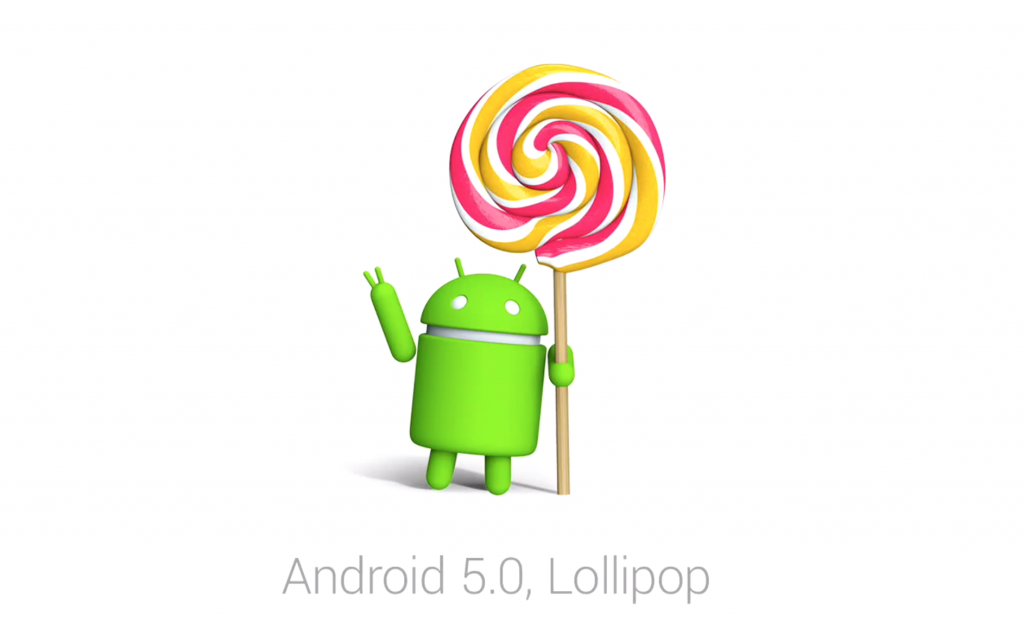
\includegraphics[width=0.5\textwidth]{figura4_lollipop.png}
				\caption{Logo oficial de Android 5.0}
			\end{figure}
		
		\newpage
		\thispagestyle{plain}
		\subsection{Arduino}
			\par
				Arduino es una plataforma de electrónica de código abierto basada en hardware y software fácil de usar. Las placas Arduino pueden leer entradas (luz en un sensor, un dedo en un botón o un mensaje de Twitter) y convertirlo en una salida, activar un motor, encender un LED y publicar algo en línea. Puede decirle a su placa qué hacer enviando un conjunto de instrucciones al microcontrolador en la placa. Para hacerlo, utiliza el lenguaje de programación Arduino (basado en ``Wiring") y el software Arduino (IDE), basado en ``Processing"
			\par \noindent
				Con los años, Arduino ha sido el cerebro de miles de proyectos, desde objetos cotidianos hasta complejos instrumentos científicos. Una comunidad mundial de fabricantes (estudiantes, aficionados, artistas, programadores y profesionales) se ha reunido en torno a esta plataforma de código abierto, sus contribuciones se han añadido a una increíble cantidad de conocimiento accesible que puede ser de gran ayuda para principiantes y expertos por igual.
			\par \noindent
				Arduino nació en el Ivrea Interaction Design Institute como una herramienta fácil para el prototipado rápido, dirigido a estudiantes sin experiencia en electrónica y programación. Tan pronto como llegó a una comunidad más amplia, la placa Arduino comenzó a cambiar para adaptarse a las nuevas necesidades y desafíos, diferenciando su oferta de simples placas de 8 bits para productos para aplicaciones IoT, wearable, impresión 3D y entornos integrados. Todos los tableros Arduino son completamente de código abierto, lo que permite a los usuarios construirlos de forma independiente y eventualmente adaptarlos a sus necesidades particulares. El software también es de código abierto y está creciendo a través de las contribuciones de los usuarios en todo el mundo.
			\begin{figure}[h]
				\centering
				
\includegraphics[width=0.4\textwidth]{figura5_arduinologo.png}
				\caption{Logo del proyecto de codigo abierto Arduino}
			\end{figure}
		
		\newpage
		\thispagestyle{plain}
		
		
		\subsubsection{Razones para utilizar Arduino}
			\begin{itemize}
				\item Económico: 
				Las placas Arduino son relativamente económicas en comparación con otras plataformas de microcontroladores. La versión menos costosa del módulo Arduino se puede ensamblar a mano, e incluso los módulos Arduino premontados cuestan menos de \$50.
				
				\item Multiplataforma: El software Arduino (IDE) se ejecuta en sistemas operativos Windows, Macintosh OSX y Linux. La mayoría de los sistemas de microcontroladores están limitados a Windows.
				
				\item Ambiente de Programación Sencilla: El software Arduino (IDE) es fácil de usar para principiantes, pero lo suficientemente flexible como para que los usuarios avanzados puedan aprovecharlo también. Para los maestros, está convenientemente basado en el entorno de programación de Procesamiento, por lo que los estudiantes que aprenden a programar en ese entorno estarán familiarizados con el funcionamiento del IDE de Arduino, adicional el lenguaje de programación es muy parecida a la C++.
				
				\item Software Extensible: El software Arduino se publica como herramientas de código abierto, disponibles para la extensión por programadores experimentados. El lenguaje puede expandirse a través de bibliotecas C ++, y las personas que quieran comprender los detalles técnicos pueden dar el salto de Arduino al lenguaje de programación AVR C en el que se basa. Del mismo modo, puede agregar código AVR-C directamente en sus programas Arduino si así lo desea.
				
				\item Hardware Extensible: 
				Los planes de las placas Arduino se publican bajo una licencia de Creative Commons, por lo que los diseñadores de circuitos experimentados pueden hacer su propia versión del módulo, ampliarlo y mejorarlo. Incluso los usuarios relativamente inexpertos pueden construir la versión del módulo para comprender cómo funciona y ahorrar dinero.
			\end{itemize}
		
		\newpage
		\thispagestyle{plain}
		
		\subsection{Componentes Electronicos}
			\subsubsection{Generalidades}
			\begin{itemize}
				\item Resistencia: 
				Son usados para establecer corrientes de operación y niveles de señal. Resistencias se utilizan en los circuitos de alimentación para reducir los voltajes al disipar la potencia, medir las corrientes y descargar los condensadores después de que se desconecta la energía. Una resistencia está hecha de elementos conductores (carbono, o una película delgada de metal o carbono, o un cable de baja conductividad), con un cable o contactos en cada extremo. Se caracteriza por su resistencia:
				$$R = V/I;$$
				
				\par \noindent
				$R$ está en ohmios para $V$ en voltios e $I$ en amperios. Esto es conocido
				como la ley de Ohm.
				
				\par \noindent
				Resistencias típicas de las más utilizadas
				tipo entrar
				valores de 1 ohmio (1) a alrededor de 10 megaohmios (10M).Las resistencias también se caracterizan por la potencia que tienen
				puede disiparse con seguridad (los más comúnmente usados son con una calificación de 1/4 o 1/8 W),su tamaño físico y otros parámetros tales como tolerancia (precisión), coeficiente de temperatura, ruido, coeficiente de voltaje (la medida en que R
				depende de V aplicado), estabilidad con el tiempo, inductancia, etc.
				
				\item Capacitor: 
				Un capacitor (el nombre antiguo era
				condensador) es un dispositivo que tiene dos cables que sobresalen
				y tiene la propiedad
				$$Q = CV$$ 
				\par \noindent
				Su forma básica es un par de placas de metal espaciadas de cerca, separados por algún material aislante. Un condensador de $C$ faradios con $V$ voltios a través de sus terminales tiene $Q$ coulombs de carga almacenada en una placa y $-Q$ en la otra. La capacitancia es proporcional al área e inversamente proporcional al espacio.
				
				\par \noindent
				Los capacitores esencialmente almacenan energía, pero es principalmente utilizado en corriente directa para filtrar picos de voltage provenientes de la fuente de la fuente de poder.
				
				\newpage
				\thispagestyle{plain}
				
				\item Inductores:
				
				
			\end{itemize}
		
		\newpage
		\thispagestyle{plain}
		
		\subsection{Sensores en General}
			\par
				Un sensor es un dispositivo capaz de detectar magnitudes físicas o químicas, llamadas variables de instrumentación, y transformarlas en variables eléctricas.
				\begin{itemize}
					\item Las variables de instrumentación pueden ser por ejemplo: temperatura, intensidad lumínica, distancia, aceleración, inclinación, desplazamiento, presión, fuerza, torsión, humedad, movimiento, pH, etc.
					
					\item Una variable eléctrica puede ser una resistencia eléctrica (como en una RTD), una capacidad eléctrica (como en un sensor de humedad o un sensor capacitivo), una tensión eléctrica (como en un termopar), una corriente eléctrica (como en un fototransistor), etc.
				\end{itemize}
			
				\noindent
				Los sensores se pueden clasificar en función de los datos de salida en: digitales y analógicos.
				
			\subsubsection{Características de los Sensores}
			
				\begin{itemize}
					\item Rango de medida: dominio en la magnitud medida en el que puede aplicarse el sensor.
					
					\item Precisión: es el error de medida máximo esperado.
					
					\item Offset o desviación de cero:  valor de la variable de salida cuando la variable de entrada es nula. Si el rango de medida no llega a valores nulos de la variable de entrada, habitualmente se establece otro punto de referencia para definir el offset.
					
					\item Linealidad o correlación lineal.
					
					\item Sensibilidad de un sensor: suponiendo que es de entrada a salida y la variación de la magnitud de entrada.
					
					\item Resolución: mínima variación de la magnitud de entrada que puede detectarse a la salida.
					
					\item Rapidez de respuesta: puede ser un tiempo fijo o depender de cuánto varíe la magnitud a medir. Depende de la capacidad del sistema para seguir las variaciones de la magnitud de entrada.
					
					\newpage
					\thispagestyle{plain}
					
					\item Derivas: son otras magnitudes, aparte de la medida como magnitud de entrada, que influyen en la variable de salida. Por ejemplo, pueden ser condiciones ambientales, como la humedad, la temperatura u otras como el envejecimiento (oxidación, desgaste, etc.) del sensor.
					
					\item Repetitividad: error esperado al repetir varias veces la misma medida.
				\end{itemize}
			
			\subsection{Termómetros}
				\par 
					El termómetro es un instrumento de medición de temperatura. Desde su invención ha evolucionado mucho, principalmente a partir del desarrollo de los termómetros electrónicos digitales.
				\par \noindent
					Inicialmente se fabricaron aprovechando el fenómeno de la dilatación, por lo que se prefería el uso de materiales con elevado coeficiente de dilatación, de modo que, al aumentar la temperatura, su estiramiento era fácilmente visible. La sustancia que se utilizaba más frecuentemente en este tipo de termómetros ha sido el mercurio, encerrado en un tubo de vidrio que incorporaba una escala graduada, pero también alcoholes coloreados en termómetros grandes.
				\par \noindent
					El creador del primer termoscopio fue Galileo Galilei; este podría considerarse el predecesor del termómetro. Consistía en un tubo de vidrio terminado en una esfera cerrada; el extremo abierto se sumergía boca abajo dentro de una mezcla de alcohol y agua, mientras la esfera quedaba en la parte superior. Al calentar el líquido, este subía por el tubo.
					
				\subsubsection{Escalas de temperatura}
					\par 
						La escala más usada en la mayoría de los países del mundo es la Celsius (\textdegree{}C) en honor a Anders Celsius (1701-1744) que se llamó centígrado hasta 1948. En esta escala, el cero (0 \textdegree{}C) y los cien (100 \textdegree{}C) grados corresponden respectivamente a los puntos de congelación y de ebullición del agua, ambos a la presión de 1 atmósfera.
					
					\newpage
					\thispagestyle{plain}
					
					\par 
						Otras escalas termométricas son:
						
						\begin{itemize}
							\item Fahrenheit (\textdegree{}F):  propuesta por Daniel Gabriel Fahrenheit en la revista Philosophical Transactions (Londres, 33, 78, 1724). El grado Fahrenheit es la unidad de temperatura en el sistema anglosajón de unidades, utilizado principalmente en Estados Unidos.
							
							\item Kelvin o temperatura absoluta, es la escala de temperatura del Sistema Internacional de Unidades. Aunque la magnitud de una unidad Kelvin (K) coincide con un grado Celsius (\textdegree{}C), el cero se ha fijado en el cero absoluto a -273,15 \textdegree{}C y es inalcanzable según el tercer principio de la termodinámica.
						\end{itemize}
				\subsubsection{Tipos de termómetros}
					\begin{itemize}
						\item Termómetro de mercurio: es un tubo de vidrio sellado que contiene mercurio, cuyo volumen cambia con la temperatura de manera uniforme. Este cambio de volumen se aprecia en una escala graduada. El termómetro de mercurio fue inventado por Gabriel Fahrenheit en el año 1714.
						
						\item Pirómetros:  termómetros para altas temperaturas, se utilizan en fundiciones, fábricas de vidrio, hornos para cocción de cerámica, etc. Existen varios tipos según su principio de funcionamiento:
						
						\begin{itemize}
							\item Pirómetro óptico: se basan en la ley de Wien de distribución de la radiación térmica, según la cual, el color de la radiación varía con la temperatura. El color de la radiación de la superficie a medir se compara con el color emitido por un filamento que se ajusta con un reostato calibrado. Se utilizan para medir temperaturas elevadas, desde 700 °C hasta 3.200 °C, a las cuales se irradia suficiente energía en el espectro visible para permitir la medición óptica.
							
							\item Pirómetro de radiación total: se fundamentan en la ley de Stefan-Boltzmann, según la cual, la intensidad de energía emitida por un cuerpo negro es proporcional a la cuarta potencia de su temperatura absoluta.
							
							\item Pirómetro infrarojos: captan la radiación infrarroja, filtrada por una lente, mediante un sensor fotorresistivo, dando lugar a una corriente eléctrica a partir de la cual un circuito electrónico calcula la temperatura. Pueden medir desde temperaturas inferiores a 0 \textdegree{}C hasta valores superiores a 2.000 \textdegree{}C.
							
							\newpage
							\thispagestyle{plain}
							
							\item Pirómetro fotoelectrónico: se basan en el efecto fotoeléctrico, por el cual se liberan electrones de semiconductores cristalinos cuando incide sobre ellos la radiación térmica.
						\end{itemize}
						
						\item Termómetro de lámina bimetálica: formado por dos láminas de metales de coeficientes de dilatación muy distintos y arrollados dejando el coeficiente más alto en el interior. Se utiliza sobre todo como sensor de temperatura en el termohigrógrafo.
						
						\item Termómetro de gas: pueden ser a presión constante o a volumen constante. Este tipo de termómetros son muy exactos y generalmente son utilizados para la calibración de otros termómetros.
						
						\item Termómetro de resistencia: consiste en un alambre de algún metal (como el platino) cuya resistencia eléctrica cambia cuando varía la temperatura.
						
						\item Termopar: un termopar o termocupla es un dispositivo utilizado para medir temperaturas basado en la fuerza electromotriz que se genera al calentar la soldadura de dos metales distintos.
						
						\item Termistor:  es un dispositivo que varía su resistencia eléctrica en función de la temperatura. Algunos termómetros hacen uso de circuitos integrados que contienen un termistor, como el LM35.
						
						\item Termómetros digitales: son aquellos que, valiéndose de dispositivos transductores como los mencionados, utilizan luego circuitos electrónicos para convertir en números las pequeñas variaciones de tensión obtenidas, mostrando finalmente la temperatura en un visualizador. Una de sus principales ventajas es que por no utilizar mercurio no contaminan el medio ambiente cuando son desechados.
						
						\item Termómetros clinicos: son los utilizados para medir la temperatura corporal. Los hay tradicionales de mercurio y digitales, teniendo estos últimos algunas ventajas adicionales como su fácil lectura, respuesta rápida, memoria y en algunos modelos alarma vibrante.
						
						\item Termógrafo: El termógrafo es un termómetro acoplado a un dispositivo capaz de registrar, gráfica o digitalmente, la temperatura medida en forma continua o a intervalos de tiempo determinado.
						
					\end{itemize}
		\newpage
		\thispagestyle{plain}
		\subsection{Impresoras 3D}
			\par
				Es necesario definir el concepto de prototipo porque es el punto de partida para el desarrollo de la tecnología de Prototipado Rapido y consecuentemente, para las impresoras tridimensionales. Podemos definir como prototipo al primer ejemplar que se fabrica de una figura, un invento o elemento físico, y sirve de modelo para fabricar otros iguales.  
			\par \noindent
				Los prototipos tiene el propósito de probar suposiciones formuladas en busca de una solución a un problema determinado. Ademas se convierten en un diseño enfocado al usuario, donde es necesario un proceso interactivo entre el propio diseñador y el consumidor. Así mismo, todos los prototipos son objetos de desarrollo de bajo costo, pero en mcuhas ocasiones la necesidad de elaborar varios prototipos o de realizar un prototipo con una estética cuidada, eleva los costes de producción. Por lo tanto, el alto coste de producción de prototipos y tiempo de ejecución de los mismos puede suponer un problema.
			\par \noindent
				Los sistemas de Prototipado Rápido surgen con la necesidad de solventar estos problemas en el uso de prototipos, se busca por lo tanto, una manera de elaborarlos con un aspecto cuidado y atractivo para el usuario, con un método de fabricación rápido y fácil de modificar, económicos y que pueden ser probados por el consumidor. Por consiguiente, esta herramienta resultará útil y funcional. Rápidamente estos sistemas de construcción aditiva partirán del desarrollo tecnológico de maquinara destinada a uso industrial. 
								
			\begin{figure}[h]
				\centering
				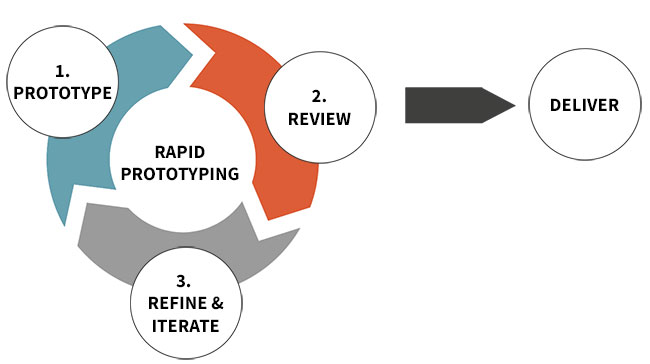
\includegraphics[width=0.7\textwidth]{figura6_rapidproto.jpg}
				\caption{Ciclo del Prototipado Rápido}
			\end{figure}
		
			\par \noindent
				El Prototipado Rápido se convierte así, en un proceso utilizado para la fabricación de prototipos, los cuales, como hemos visto, son objetos que no estan diseñados a uso final, sino más bien a modo de prueba de diseño.
				
			\newpage
			\thispagestyle{plain}
			\par \noindent
				La impresión 3D, también conocida como impresión tridimensional, es un método para
				producir objetos tridimensionales con un aparato tecnológico al colocar varias capas
				bidimensionales de cierto material una sobre la otra. El proceso es similar a la impresión
				bidimensional en la cual se coloca tinta sobre papel, sin embargo, en la impresión
				tridimensional se coloca plástico sobre una superficie que nos permite fabricar objetos de tres
				dimensiones. Esta tecnología se utiliza principalmente en la producción de prototipos durante
				el diseño de algún nuevo producto.
			\par \noindent
				Durante los últimos años, la tecnología de impresión tridimensional ha avanzado de
				manera exponencial. Este tipo de impresoras se han vuelto cada vez más accesibles y por ello
				ahora es común encontrarlas en fábricas, industrias, instituciones educativas, instituciones de
				investigación e inclusive para uso personal.
			
			\subsubsection{Técnicas}
				\begin{itemize}
					\item SLA (Estereografía): Se basa en las propiedades de una resina fotosensible que se solidifica mediante la proyección de un láser (UV) de frecuencia y potencia concreta.
					
					\begin{figure}[h]
						\centering
						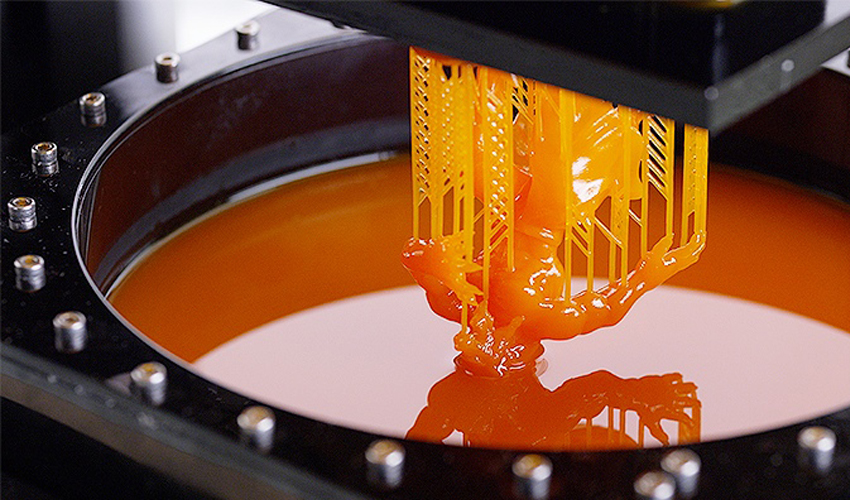
\includegraphics[width=8cm, height=6cm]{figure7_slaprint.jpg}
						\caption{Resultado de impresión tridimensional SLA}
					\end{figure}
					
					\item SLS (Sintetización selectiva laser): En vez de emplear un fotopolímero como ocurre con la SLA, para sintetizarlo, utiliza un compuesto en polvo de diversas clases, normalmente microesferas de poliamida junto con un láser que causa que las partículas se fusionen y solidifiquen. 
					
					\newpage
					\thispagestyle{plain}
					
					\begin{figure}[h]
						\centering
						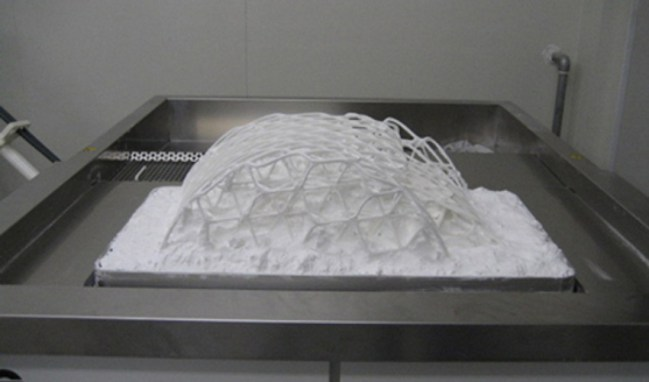
\includegraphics[width=8cm, height=6cm]{figure8_slsprint.jpg}
						\caption{Resultado de impresión tridimensional SLS}
					\end{figure}
					
					\item FDM (Modelado por disposición de hilo fundido): Consiste en la deposición por capas de material normalmente construido por filamentos de polímeros termoplásticos, que se funden y se extruyen por medio de una boquilla, solidificándose cuando salen de dicha boquilla al exterior. Esta técnica es la que utilizaremos en este trabajo.
					
					\begin{figure}[h]
						\centering
						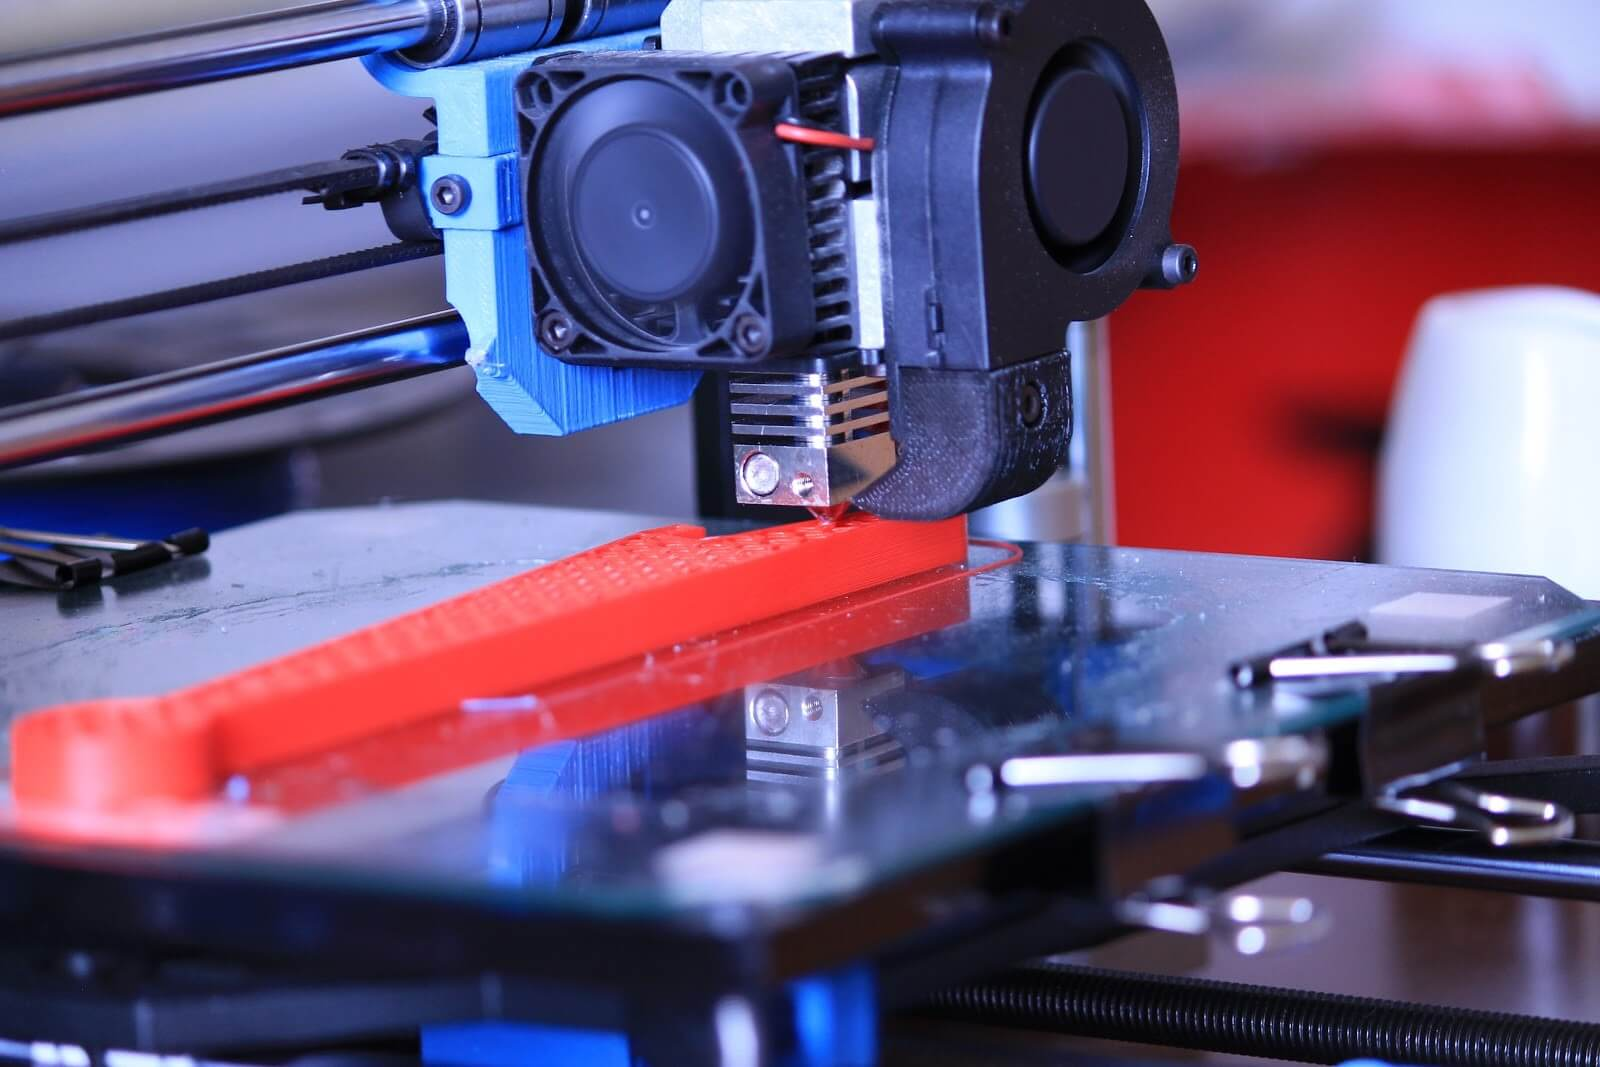
\includegraphics[width=8cm, height=6cm]{figure9_fdmprint.jpg}
						\caption{Resultado de impresión tridimensional FDM y Vista de una boquilla o extrusor}
					\end{figure}
					
					\item SGC (Fotopolimerización): Al igual que en la estereolitografía, la fotopolimerización se basa en la solidificación de
					un fotopolímero o resina fotosensible, sin embargo, en el proceso de
					fotopolimerización se irradia, con una lámpara de UV en vez de con un láser
					ultravioleta. Por lo tanto, necesita una única operación junto con máscaras creadas
					con tinta electroestática en una placa de vidrio.
					
					\newpage
					\thispagestyle{plain}
					
					\begin{figure}[h]
						\centering
						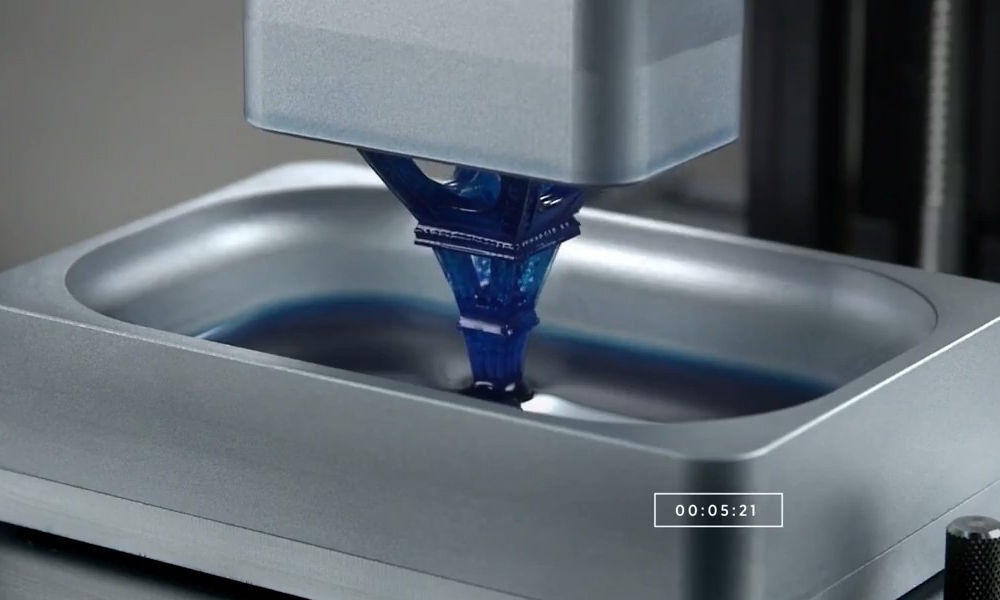
\includegraphics[width=8cm, height=6cm]{figura14_sgcprint.jpg}
						\caption{Resultado de impresora SGC}
					\end{figure}
					
					\item DMLS (Direct Metal Laser Sintering): fue patentado por las empresas ERD y EOS
					(Alemania) en 1994, incluso las primeras investigaciones comenzaron en los años 70. 
					
					
					\par \noindent
						La plataforma en la que se realiza la impresión está compuesta de 2 recipientes, cada
						uno activado por un pistón. El primero es recubierto de polvo metálico mientras que el
						segundo se encuentra vacío y situado al nivel de la plataforma. El proceso de
						impresión empieza añadiendo una fina capa de polvo (de una altura máxima
						determinada por el software de la impresora) en el recipiente vacío. El láser de fibra
						fusiona el polvo metálico. Una vez que la materia se consolida, una segunda capa de
						polvo es aplicada con la ayuda del sistema de pistones, y así sucesivamente hasta la
						creación completa de la pieza.
						
					\begin{figure}[h]
						\centering
						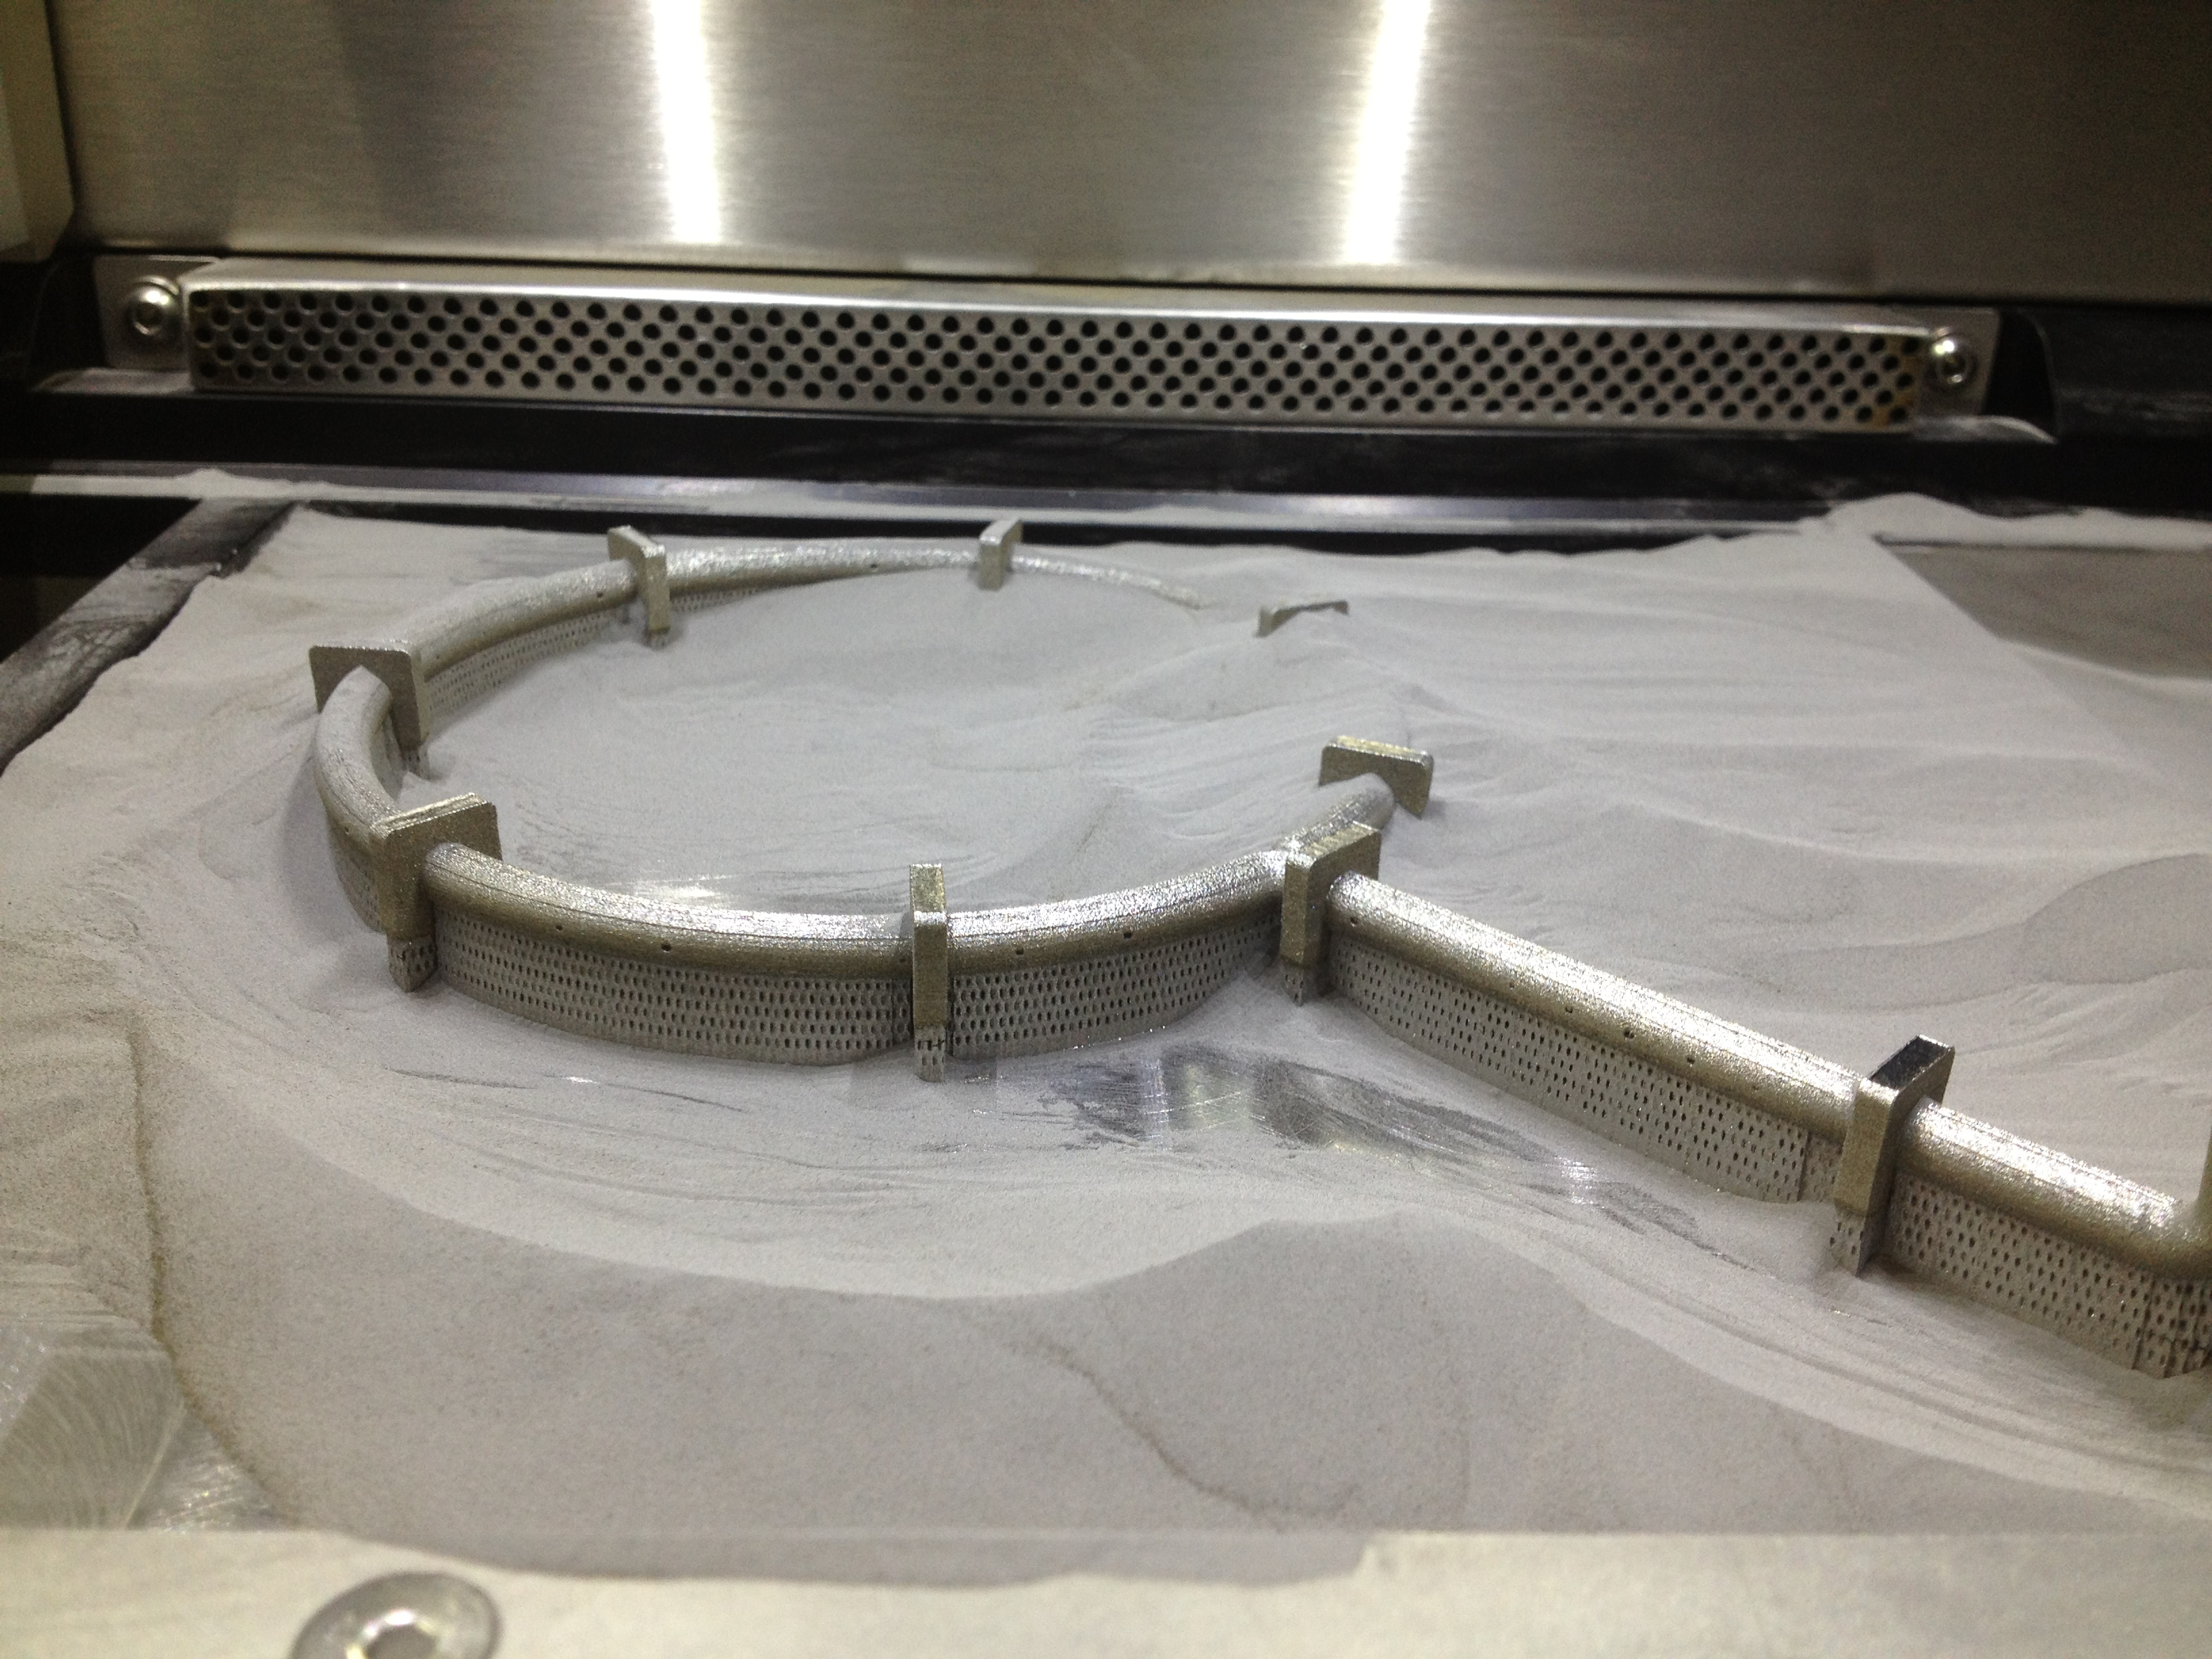
\includegraphics[width=8cm, height=6cm]{figure10_dmlsprint.jpg}
						\caption{Resultado de impresión tridimensional DMLS}
					\end{figure}
				
				\newpage
				\thispagestyle{plain}
						
					\item CLG (Cerámica láser gelificante): La materia prima que se utiliza en la cerámica láser gelificante, es un polvo cerámico
					con un compuesto inorgánico soluble en agua que forma una pasta cerámica. Este
					compuesto es expuesto a un láser de 4W que evapora el agua en una zona
					determinada de la capa, la cual se gelifica localmente para formar capa a capa una
					pieza cerámica en crudo. 
					
					
					
					\begin{figure}[h]
						\centering
						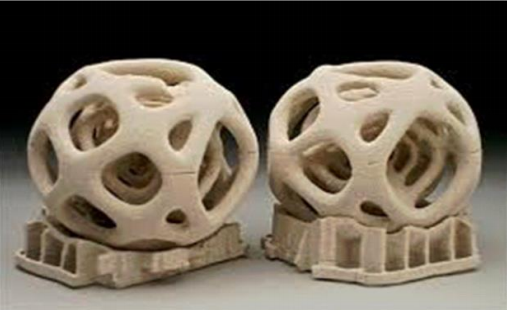
\includegraphics[width=8cm, height=6cm]{figura11_ceramicprint.png}
						\caption{Resultado de impresión tridimensional CLG}
					\end{figure}
					
					\item LOM (Fabricación por Corte Laminado): El proceso consiste en cortar, posicionar y pegar o unir láminas de material como
					papel, arena, cerámica y composites.
					
					\begin{figure}[h]
						\centering
						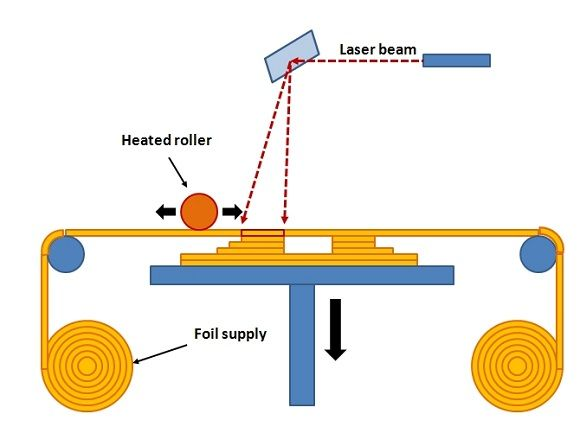
\includegraphics[width=8cm, height=6cm]{figura12_lomprint.jpg}
						\caption{Arquitectura de impresora LOM}
					\end{figure}
					
				\end{itemize}
		\newpage
		\thispagestyle{plain}
		\subsection{Equipos utilizados para la calibración de termómetros}
		

				
			
			